\section{Theoretical Analysis}  \label{sec:analysis}

\paragraph{} First of all, we need to analyse the circuit in general. It has thirteen meshes, of which four are elementar,
nine nodes and eleven branches (seven resistors, one independent voltage source $V_s$, one voltage controlled current
source $I_b$, one current controlled voltage source $V_d$ and one capacitor with charge $C$.

%%%%%%%%%%%%%%PRIMEIRO PONTO DA TEÓRICA%%%%%%%%%%%%%%%%%%%%%%%
\subsection{The voltages in all nodes and the currents in all branch for $t<0$} \label{2.1}

\paragraph{} According to information provided in the circuit, when $t<0$, $u(t)=0$. Therefore, $V_s(t)=V_s$, so that means $V_s(t)$ is constant.
We also assume that the capacitor already has a static value,
so the voltage in nodes 6 and 8 is the same, so there is no current passing through this branch and we have what is called an open
circuit. In order to determine the currents and voltages in the nodes we use the Node Voltage Method. When we use the term
node voltage, we are referring to the potential difference between two nodes of a circuit. This is still a voltage,
it's not anything too strange. We start by labelling the nodes with numbers and assigning each with its own variable,
$V_1$, $V_2$, etc. Then, we select one of the nodes in the circuit to be the reference node and call this reference
node the ground node. The potential of the ground node is defined to be $0 V$. The choice of the reference node is
somewhat arbitrary, but it's always best to choose it based on its connections to voltage sources, because by this
selection we already know the node voltages of other nodes, i.e. the ones that the reference node is connected to
them by voltage sources. In our case we already have the ground in the circuit, so we use that. With this information
we are able to obtain the following equations:

\begin{center}
  \begin{gather*}
    V_s=V_1 \\ V_b=V_2-V_5
  \end{gather*}
\end{center}

\par We use the previous equations to facilitate the equations referring
to the Node Voltage Method and we get these equations:

\begin{center}
  \begin{gather*}
    V_s = V_1 \\
    V_1(-G_1)+V_2(G_1+G_2+G_3)+V_3(-G_2)+V_5(-G_3)=0 \\
    V_2(-G_2-K_b)+V_3G_2+V_5K_b=0 \\
    V_2(-G_3)+V_5(G_3+G_5+G_4+\frac{1}{K_d})+V_6(-G_5)+V_8(\frac{-1}{K_d})=0 \\
    V_2K_b+V_5(-K_b+-G_5)+V_6(G_5)=0 \\
    V_7(G_6-G_7)+V_8G_7=0 \\
    V_5+V_7(K_dG_6)-V_8=0
  \end{gather*}
\end{center}


where G is the conductance of the resistors, given by the relation $G = \frac{1}{R}$. Solving these equations in
order of $V_n$, n = \{1,2,3,5,6,7,8\}, allows to then simply calculate the currents and voltages in play in
this circuit, using Ohm's Law, among others. Octave was used to compute the solution of this 7 equation system,
giving the following solutions:

\begin{table}
  \centering
  \begin{tabular}{|l|r|}
    \hline
    {\bf Name} & {\bf Value [A or V]} \\ \hline
    Ic & 0.0\\ \hline 
Ib & -0.00139222950\\ \hline 
I1 & -0.00132891839\\ \hline 
I2 & -0.00139222950\\ \hline 
I3 & -0.00006331111\\ \hline 
I4 & 0.00097696107\\ \hline 
I5 & 0.00139222950\\ \hline 
I6 & 0.00035195732\\ \hline 
I7 & 0.00035195732\\ \hline 
V1 & 5.0737445952\\ \hline 
V2 & 3.71767606204\\ \hline 
V3 & 0.92740888235\\ \hline 
V5 & 3.91334407167\\ \hline 
V6 & 8.13366324395\\ \hline 
V7 & 0.72653594426\\ \hline 
V8 & 1.09343609721\\ \hline 
Id & 0.00035195732\\ \hline 

  \end{tabular}
  \caption{Current and voltage in each node}
  \label{tab:op}
\end{table}


%%%%%%%%%%%%%%%%%%%%SEGUNDO PONTO DA TEÓRICA%%%%%%%%%%%%%%%%%%%%%%%%%%%
\subsection{The equivalent resistance $R_{eq}$} \label{2.2}


\paragraph{} To learn the equivalent resistance $R_{eq}$ as seen from the capacitor terminals, we make $V_s=0 V$ and
replace the capacitor with a voltage source $V_x=V_6-V_8$ ($V_6$ and $V_8$ are the voltages
in the nodes 6 and 8 obtained in \ref{2.2}). This way, we apply again the Node Voltage Method to
determine $I_x$ and $V_x$, in order to calculate the equivalent resistance $R_{eq} = \frac{V_x}{I_x}$ and then the time constante
$\tau$. Written below are the equations for the nodes:

\begin{center}
  \begin{gather*}
    V_1=V_0 \\
    V_1G_1+V_2(-G_1-G_2-G_3)+V_3G_2+V_5G_3=0 \\
    V_2(G_2+K_B)-V_3G_2-V_5K_b=0 \\
    -V_1G_1+V_2G_1+V_5G_4+V_7G_6=0 \\
    V_5+V_7K_dG_6-V_8=0 \\
    V_6-V_8=V_x \\
    V_7(-G_6-G_7)+V_8G_7=0 \\
  \end{gather*}
\end{center}


\paragraph{} Solving this system of linear equations in $Octave$ we get:

\begin{table}[h]
  \centering
  \begin{tabular}{|l|r|}
    \hline
    {\bf Name} & {\bf Value [A or V]} \\ \hline
    Ib & -0.00139222950\\ \hline 
I1 & 0.00000000000\\ \hline 
I2 & 0.00000000000\\ \hline 
I3 & 0.00000000000\\ \hline 
I4 & 0.00000000000\\ \hline 
I5 & -0.00227796363\\ \hline 
I6 & 0.00000000000\\ \hline 
Id & -0.00000000000\\ \hline 
V1 & 0.0000000000\\ \hline 
V2 & 0.00000000000\\ \hline 
V3 & 0.00000000000\\ \hline 
V5 & 0.00000000000\\ \hline 
V6 & 7.04022714674\\ \hline 
V7 & 0.00000000000\\ \hline 
V8 & 0.00000000000\\ \hline 
$R_{eq}$ & 3031.33870093000\\ \hline 

  \end{tabular}
  \caption{Table with the values of current and voltage}
  \label{tab:op2}
\end{table}


\paragraph{} Using the values obtained, we can find out the expression for
voltages in the terminal of the capacitor. The solution has two components,
the natural solution and the forced solution. Doing this procedure allows to easily find out
the natural solution of the circuit.


%%%%%%%%%%%%%%%%%%%%TERCEIRO PONTO DA TEÓRICA%%%%%%%%%%%%%%%%%%%%%%%%%%%
\subsection{The Natural solution} \label{2.3}

\paragraph{} The natural solution depends on the initial voltage, equivalent resistance and
capacitance of the capacitor. By solving the first order differential equation given by analyzing the circuit,
we get the following natural solution:

\begin{center}
  \begin{gather*}
    v_{6n}(t)=V_x e^\frac{-t}{R_{eq}C}
  \end{gather*}
\end{center}



\par Plotting the expression in a graph using the range of $[0,20]ms$ we get:

\begin{figure}[h]
  \centering
  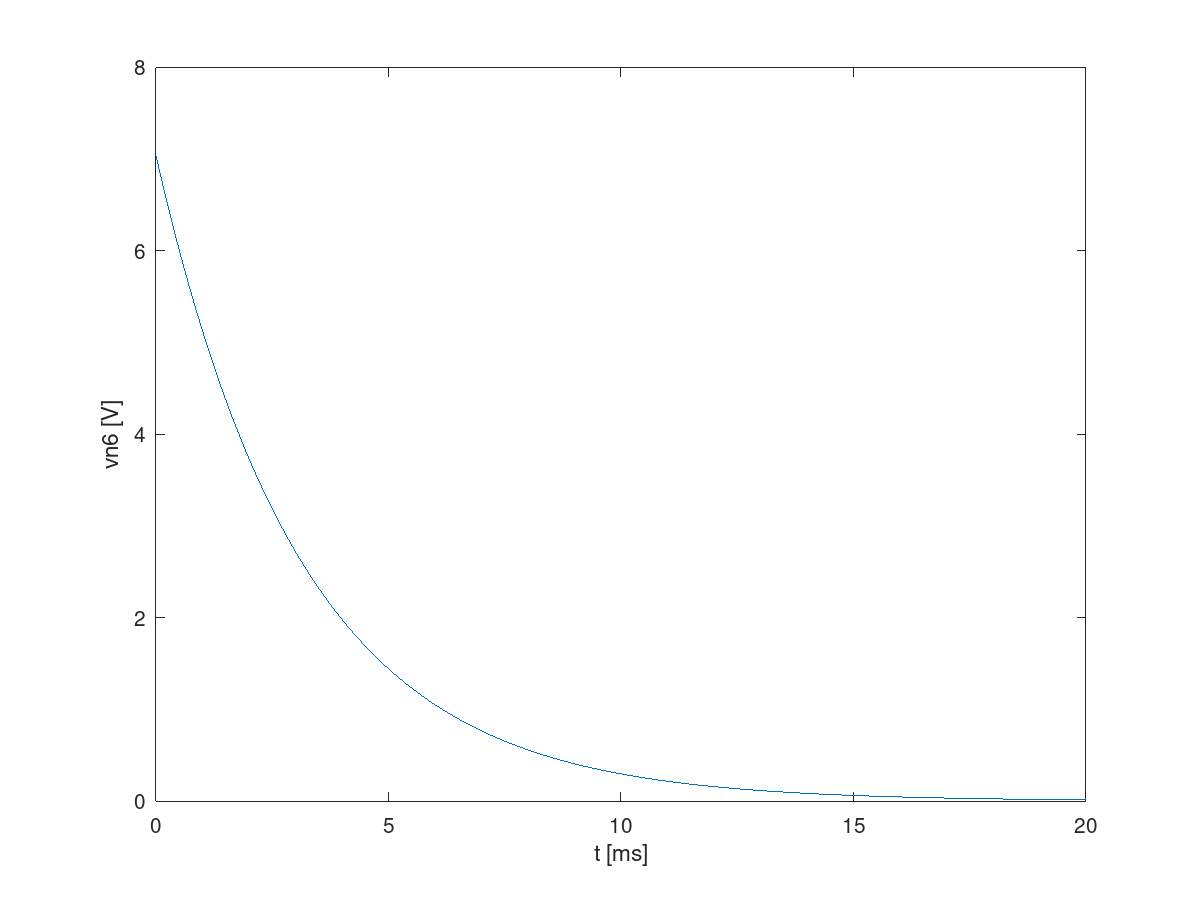
\includegraphics[width=9cm,height=5cm,keepaspectratio]{v6natural.png}
  \caption{Representation of the Natural Solution in $[0,20]ms$}
\end{figure}




%%%%%%%%%%%%%%%%%%%%QUARTO PONTO DA TEÓRICA%%%%%%%%%%%%%%%%%%%%%%%%%%%
\subsection{The Forced solution} \label{2.4}

\paragraph{} Now that we have the expression for the natural solution we need
to find the expression of the forced solution in order to obtain the total solution of the circuit. This solution depends on the voltage
source, equivalent resistance and the capacitance of capacitor.

\begin{center}
  \begin{gather*}
    v_{6f}(t)= sin(2\pi f t)
  \end{gather*}
\end{center}

\paragraph{} To obtain this expression for $f=1kHz$,we start by using a phasor voltage source $V_s=1$, replacing C with its impedance $Z_c$ and using
Node Analysis once again to determine the phasor voltages in each node. We get the following expressions:

\begin{gather*}
  \widetilde{V_s} = e^{-j\frac{\pi}{2}} = V_1 \\
  -V_1G_1 +V_2G_1 + V_5G_4 + V_7G_6 = 0 \\
  V_1G_1 + V_2(-G_1-G_2-G_3)+V_3G_2+V_5G_3 = 0 \\
  V_2 (G_2 + K_b) -V_3G_2 -V_5K_b = 0 \\
  -V_2K_B+V_5(K_b + G_5) + V_6(-G_5 -jwC) + V_8(jwC) = 0 \\
  V_7 (-G_6-G_7) + V_8G_7 = 0 \\
  V_5 + V_7(K_dG_6) - V_8 = 0 \\
\end{gather*}

\begin{table}[h]
  \centering
  \begin{tabular}{|l|l|l|}
    \hline
    {\bf Name} & {\bf Amplitude } & {\bf Angle [rad]} \\ \hline
    $\tilde{V_1}$ & 1.0000000 & -1.5707963\\ \hline 
$\tilde{V_2}$& 0.9550715 & -1.5707963\\ \hline 
$\tilde{V_3}$ & 0.8626260 & -1.5707963\\ \hline 
$\tilde{V_4}$ & 0.0 & 0.0\\ \hline 
$\tilde{V_5}$ & 0.9615543 & -1.5707963\\ \hline 
$\tilde{V_6}$& 0.6107405 & 1.7122338\\ \hline 
$\tilde{V_7}$ & 0.4046424 & 1.5707963\\ \hline 
$\tilde{V_8}$ & 0.6089866 & 1.5707963\\ \hline 

  \end{tabular}
  \caption{Complex amplitudes and angles in each node for the forced solution}
  \label{tab:analise4}
\end{table}


%%%%%%%%%%%%%%%%%%%%QUINTO PONTO DA TEÓRICA%%%%%%%%%%%%%%%%%%%%%%%%%%%

\subsection{The Final Total Solution} \label{2.5}

\paragraph{} The Final Total Solution is the sum of the Natural Solution and the Forced Solution,
obtained in \ref{2.3} and \ref{2.4} respectively:


\begin{center}
  \begin{gather*}
    v_{6}(t)= V_x e^\frac{-t}{R_{eq}C}+sin(2\pi f t)
  \end{gather*}
\end{center}

\paragraph{} Plotting the expression in a graph we get:


\begin{figure}[h]
  \centering
  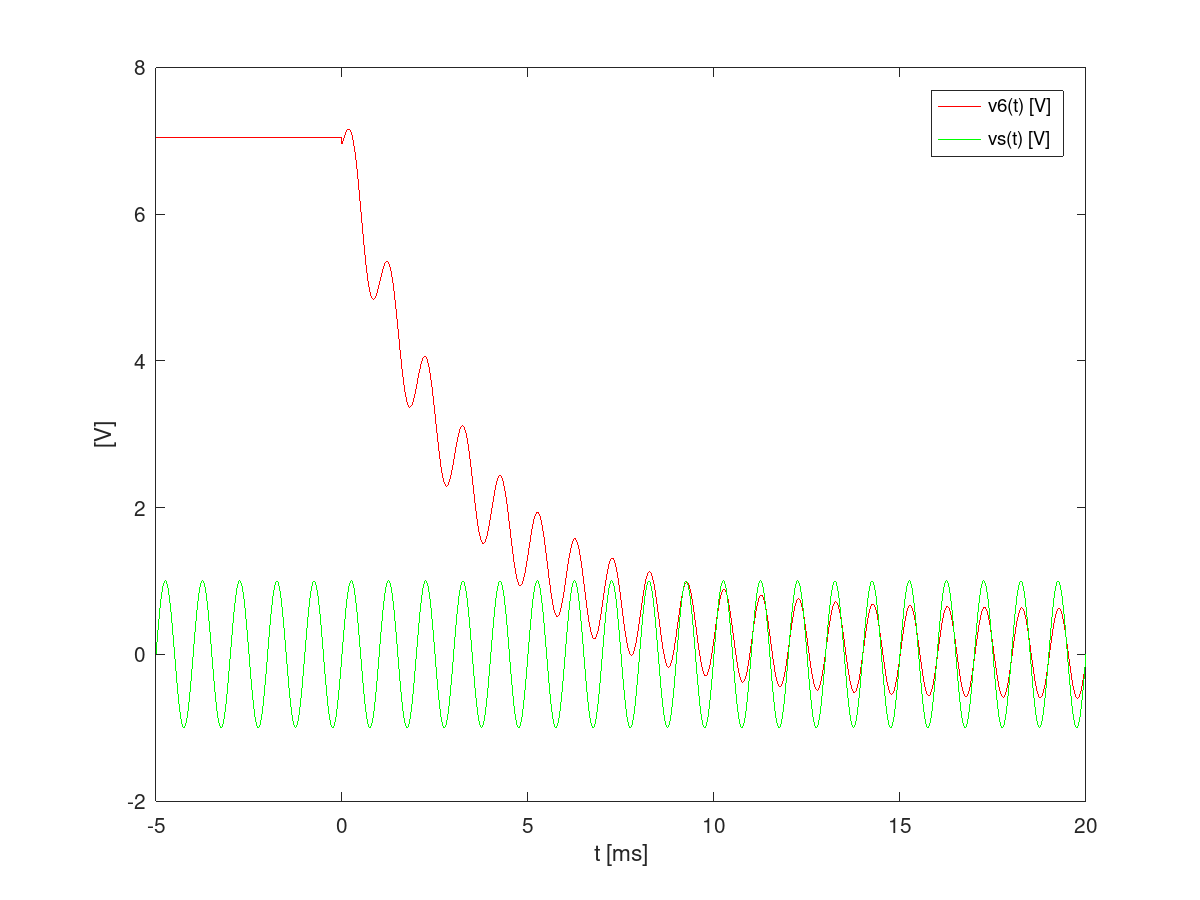
\includegraphics[width=9cm,height=5cm,keepaspectratio]{total.png}
  \caption{Representation of the Final Total Solution in $[-5,20]ms$}
\end{figure}



%%%%%%%%%%%%%%%%%%%%SEXTO PONTO DA TEÓRICA%%%%%%%%%%%%%%%%%%%%%%%%%%%

\subsection{The Final Total Solution for frequency range $0.1Hz$ to $1MHz$} \label{2.6}

\paragraph{} Now we plot the graph of $V_s$, $V_6$ and $V_C = V_6 - V_8$ (db) in function of the
frequency (using a logarithmic scale) and in function of the phase (degrees). We obtained the following
graphics:

\begin{figure}[h]
  \centering
  \begin{subfigure}{0.23\textwidth}
    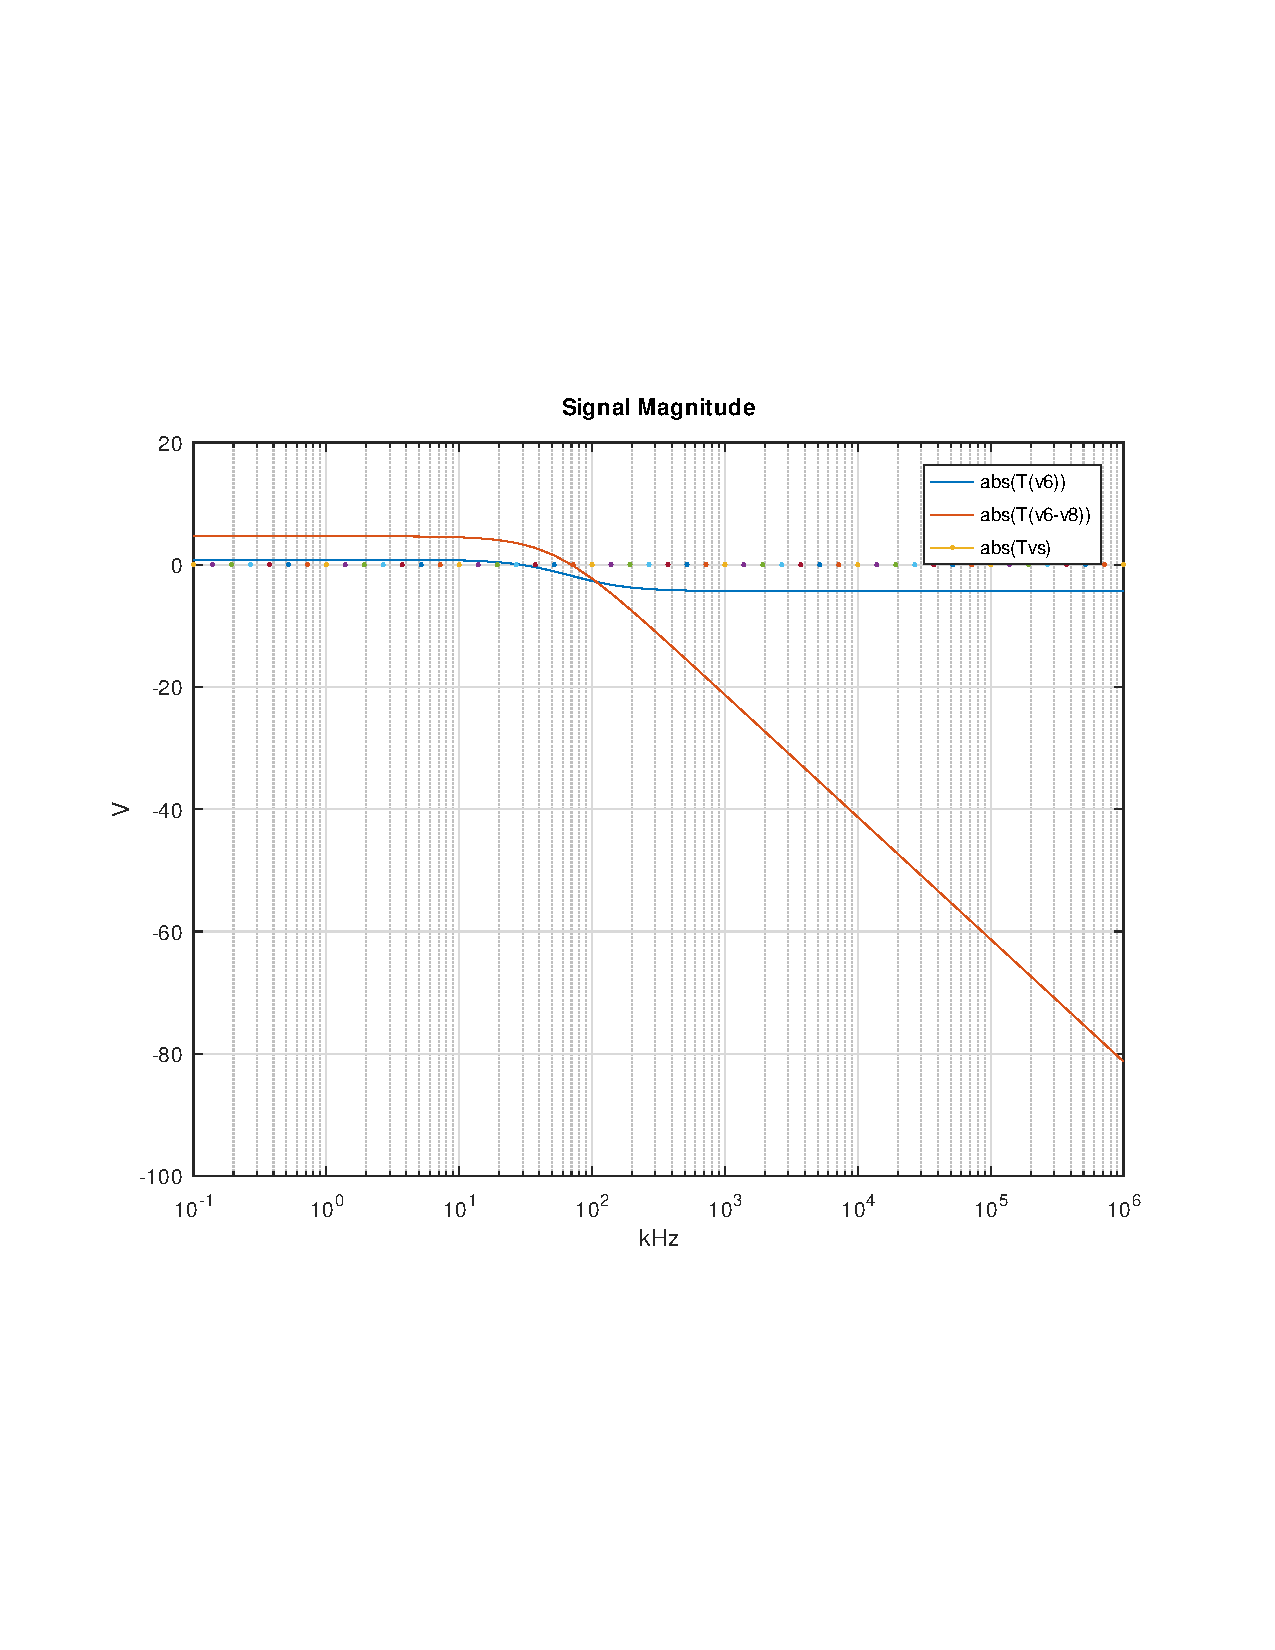
\includegraphics[width=\linewidth, clip]{../mat/Transmagnitude.pdf}
    \label{fig:PStime}
  \end{subfigure}
  \begin{subfigure}{0.23\textwidth}
    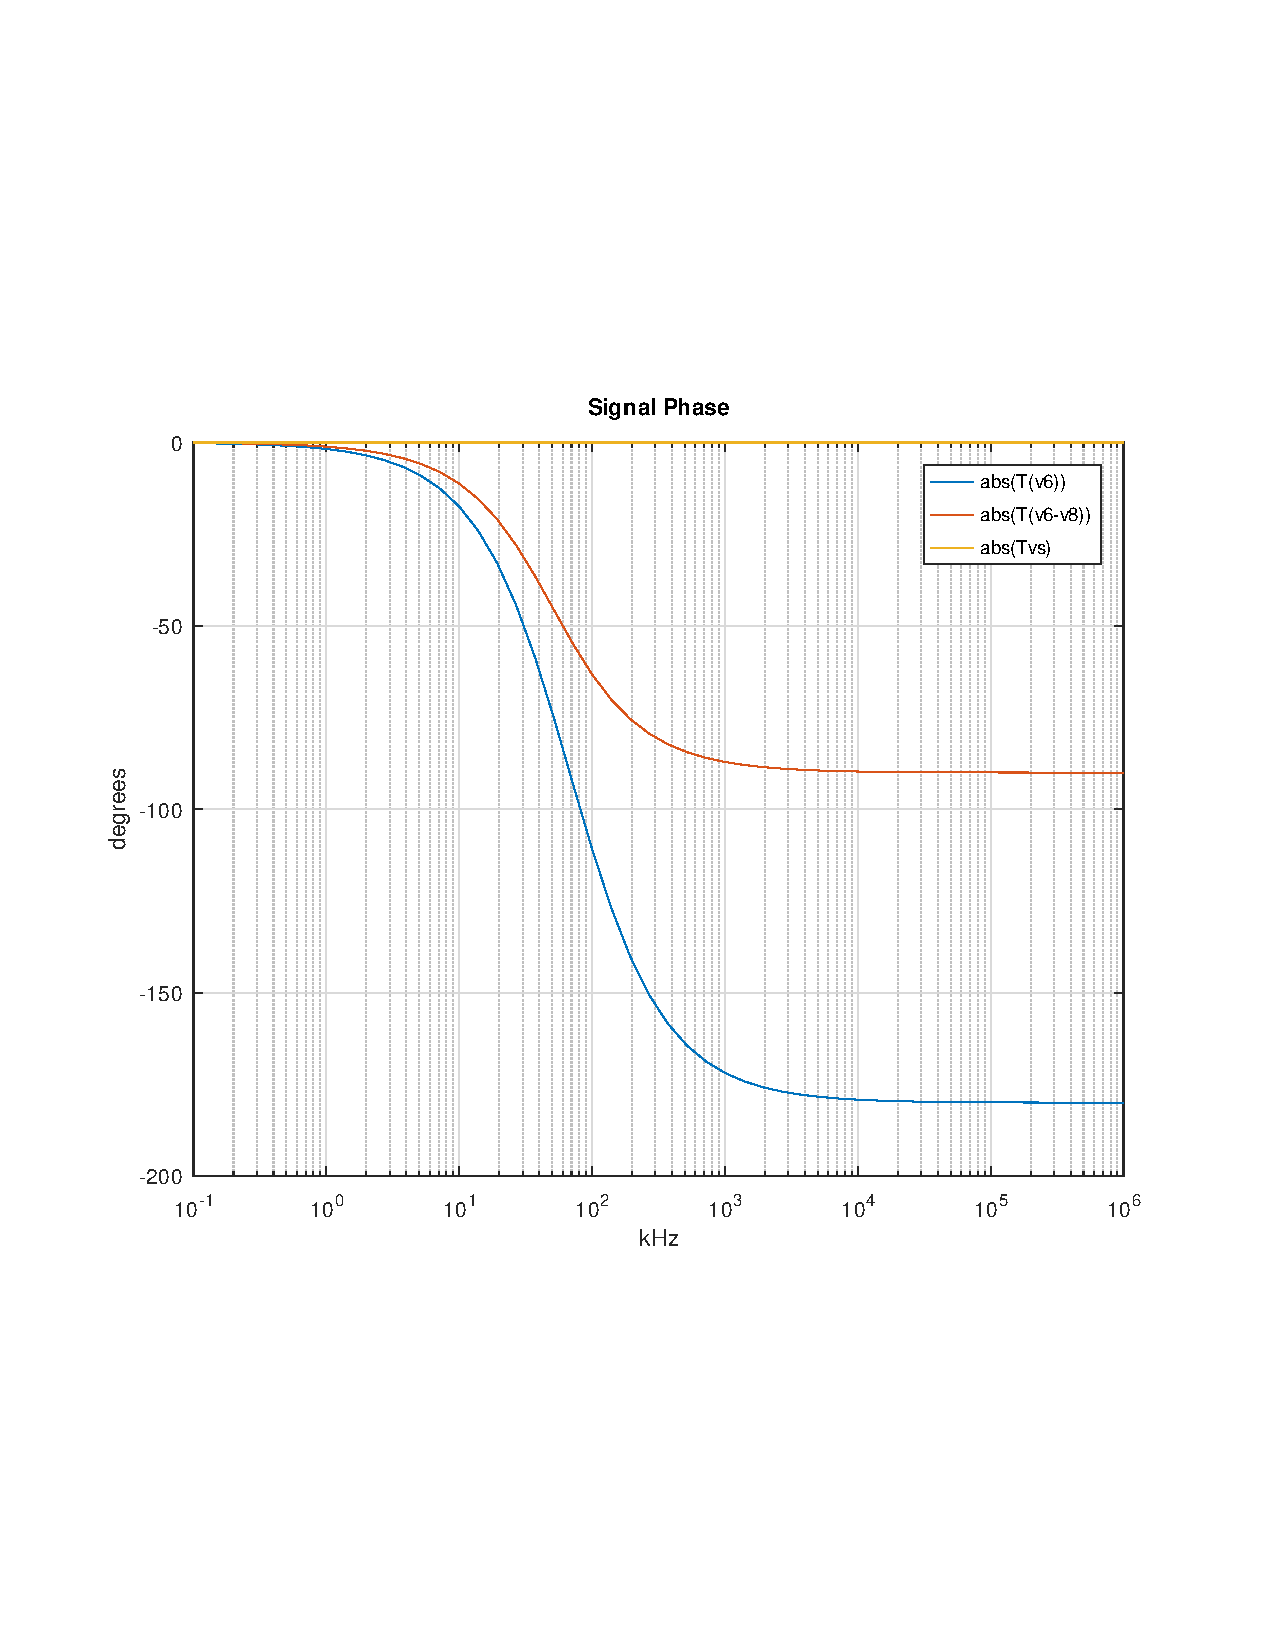
\includegraphics[width=\linewidth, clip]{../mat/Transphase.pdf}
    \label{fig:PSciclo}
  \end{subfigure}

  \caption{\small V(f) with frequency range $0.1Hz$ to $1MHz$ (left) and V(p) (right).}
  \label{maquina}
\end{figure}

%explicar o da magnitude
\paragraph{} Comparing the $V(f)$ graphs,
they are very distinct from each other.
The magnitude of $V_s(f)$ is always $\approx 0$. It never changes because it's
an imposed voltage from the voltage source. $V_c(f)$ has a steady positive value for a while
and then rapidly decreases permanently. $V_6(f)$ starts off constant and positive then softly decreases
and stabilizes at a negative constant value. With big values of frequency, of the voltage $|V_c|$ in the capacitor also increases.
Consequently, the voltage $|V_6|$ will have a bigger value. However, this value will be constant due to the exponential contribution $ \exp(\frac{-t}{R_{eq}C})$.


%explicar o da fase 

\paragraph{} Now looking at the $V(p)$ graphs, they are also quite different. While $V_s(p)$ is always
$\approx 0$ , both $V_C(p)$ and $V_6(p)$ start off at $\approx 0$ but then rapidly decrease to a constant negative value ($\approx -180o $ and $\approx -85o$ respectively)




